% This file should be replaced with your file with an thesis content.
%=========================================================================
% Authors: Michal Bidlo, Bohuslav Křena, Jaroslav Dytrych, Petr Veigend and Adam Herout 2019

% For compilation piecewise (see projekt.tex), it is necessary to uncomment it and change
% \documentclass[../projekt.tex]{subfiles}
% \begin{document}


\chapter{Introduction}

Although more than 30 years have passed since the invention of the web back in 1989 \cite{WWWProposal}, it is still an integral part of our lives, possibly more than ever before. People worldwide use the web daily to work, learn, consume content and connect with others. Every day our smartphones, tablets, laptops, or even smartwatches and fridges connect to the web.

This diverse ecosystem of devices created a need to identify users who use them uniquely. The ability to uniquely identify a user on a single device or across multiple devices allows applications to personalize the content they provide or improve their security.
One of the methods of user identification is browser fingerprinting, the collection of data from the browser to create a fingerprint of the device. Just as a person's fingerprint can uniquely identify that specific person, given that we have enough data, we can uniquely identify a device and its user and act on this information.

However, gathering this kind of data can be considered a violation of privacy \cite{WP224Fingerprinting}, which is the primary motivation behind creating privacy-first browsers and browser extensions to fight against fingerprinting. One of the browser extensions set on improving privacy is JShelter\footnote{JShelter is an anti-malware browser extension to mitigate potential threats from JavaScript, including fingerprinting \cite{JShelterHome} (Available at \url{https://jshelter.org/}).} which focuses on preventing active fingerprinting.

Active fingerprinting is a method of obtaining a fingerprint, typically by running JavaScript code to collect data from browser APIs \cite{FingerprintingSurvey}. The other variant is passive fingerprinting, in which the data is collected solely from network traffic, for example, HTTP headers.

This work aims to design and implement a browser extension to prevent the collection of passive fingerprints by altering data in HTTP requests and explore possibilities of integrating this protection into JShelter. It is important to note that the altered data must be consistent with the data obtainable through active fingerprinting methods. Otherwise, the fingerprinting application could recognize an attempt to mitigate the effects of fingerprinting.

Fingerprinting is an ever-evolving field. Chapter \ref{Chapter:BrowserFingerprinting} describes its nature, history, and different approaches to collecting a fingerprint. The last two sections of chapter \ref{Chapter:BrowserFingerprinting} provide an outlook on threats and opportunities fingerprinting brings to the table because, as we know, nothing is purely black and white.

As this work explores the capabilities of mitigating fingerprinting with the help of browser extensions, the following chapter \ref{Chapter:Extensions} gives the reader an insight into the inner working of extensions.

Finally, the last chapter \ref{Chapter:Design} proposes a design of passive fingerprinting protection that works consistently with active solutions to keep user-observable side effects to a minimum.

\section{Definitions}

\begin{itemize}
	\item \textbf{Fingerprint}: A collection of device-specific characteristics gathered for the purpose of identification.
	\item \textbf{Fingerprinting}: The process of collecting the device information (data) to compute a fingerprint. Terms fingerprinting, device fingerprinting, and browser fingerprinting will be used interchangeably in the following chapters.
	\item \textbf{Fingerprinter}: An application performing fingerprinting, typically on a third-party remote server.
\end{itemize}

% -------------------------------------------------------------------- %

\chapter{Web browsers}
% TODO: Chapter description. The part below is copied from the old chapter "web extensions".

In this chapter, the first section, \ref{Section:WebExtensionsAPI}, describes the WebExtensions API exposed by a browser to give extensions more capabilities. Recently, significant changes to the ecosystem of extensions were announced with the introduction of Manifest V3, described in section \ref{Section:ManifestV3}. The last section, \ref{Section:JShelter}, is dedicated to the JShelter extension on which this work builds.

\section{History of web browsers}

Web browsers have come a long way since the early days of the World Wide Web. From their humble beginnings as basic applications for viewing text-only web pages, modern browsers have evolved into the powerful tools we know today. Following paragraphs outline the evolution of browsers, highlighting a few of the most significant features added over the years.

The first browser, named WorldWideWeb\footnote{\url{https://worldwideweb.cern.ch}}, was created at CERN by Tim Berners-Lee only a year after he published the first World Wide Web proposal \cite{WWWProposal}. The very early browser aimed to demonstrate how the user-facing layer of the WWW (browsers) could work in the future. The browser was only available on the NeXTSTEP\footnote{\url{https://en.wikipedia.org/wiki/NeXTSTEP}} operating system and had limited features.

One of the earliest features added to browsers was support for images. The Mosaic browser\footnote{\url{https://en.wikipedia.org/wiki/Mosaic_(web_browser)}}, released in 1993, was the first to allow users to view images on the web, followed by support for tables, which allowed for more complex web page layouts.

As the web gained popularity, developers needed a way to make web pages more interactive and dynamic. The birth of JavaScript programming language addressed this need. JavaScript was first introduced in 1995\footnote{\url{https://en.wikipedia.org/wiki/Netscape_Navigator_2}} by Netscape Communications Corporation to add interactivity to static HTML pages. Since then, it has become one of the world's most widely used programming languages, with a vast ecosystem of libraries and frameworks\footnote{\url{https://www.npmjs.com/}}.

Nowadays, web browsers expose a variety of JavaScript APIs that allow web developers to interact with the browser and its underlying components, such as the operating system or even the hardware. While it is true that these APIs gave the developers much-needed possibilities, they come at the cost of compromised privacy, described in detail in the following chapters.

\section{JavaScript}

In its original form, JavaScript is a client-side language executed in the user's web browser rather than on a web server \cite{JSDefinitiveGuide}. It allows applications to respond to user actions in real time without making a round trip to the server. However, the rise of popularity and the fact that JavaScript is a relatively developer-friendly language meant that, eventually, runtimes that allowed running JavaScript outside the browser emerged. The most popular JavaScript runtimes include Node.js\footnote{\url{https://nodejs.org/}}, Deno\footnote{\url{https://deno.land/}}, or Bun\footnote{\url{https://bun.sh/}}.

\subsection{ECMAScript}

As the web was rapidly gaining popularity, developers started using JavaScript to create dynamic and interactive web pages. However, there was no standardization for the language, meaning different browsers implemented JavaScript differently. This made it difficult for developers to create web applications that worked consistently across different platforms and browsers \cite{JSDefinitiveGuide}.

In 1996, Netscape Communications Corporation, the company behind the Netscape Navigator web browser, submitted JavaScript to ECMA International\footnote{\url{https://www.ecma-international.org/}}. This standards organization develops and maintains standards for several technologies, including programming languages. The goal was to create a standardized language version that could be implemented across different platforms and browsers.

ECMA International established a committee to develop a standardized scripting language, which was initially called ECMA-262. The standard's first version, ECMAScript 1, was released in June 1997. Since then, ECMAScript has undergone several revisions, the latest being ECMAScript 2022. Each standard version adds new features and capabilities to the language while maintaining backward compatibility with previous versions \cite{JSDefinitiveGuide}.

Although ECMAScript is technically the correct name for the language, JavaScript is used in the following chapters as the industry uses this name predominantly.

\subsection{Web APIs}

Web applications can use JavaScript Web APIs to interact with various web browser features and functionality. The number of available APIs depends on the browser. For example, at the time of the writing, Firefox had more than 100 APIs\footnote{\url{https://developer.mozilla.org/en-US/docs/Web/API}}, with more APIs still being added. Here is a short selection of Web APIs important to the topic of this thesis \cite{SecurityWebDevs, SchauerDP}:

\begin{itemize}
	\item \textbf{Canvas API}: Provides a way to dynamically create and manipulate graphics and animations in a web page using JavaScript.
	\item \textbf{Navigator}: Provides information about the web browser or user agent in which the code runs.
	\item \textbf{Web Audio API}: Provides advanced audio processing and synthesis capabilities, allowing developers to create interactive audio experiences on the web.
	\item \textbf{WebGL}: Allows for creating and rendering interactive 3D and 2D graphics within a web browser using the computer's graphics hardware capabilities.
\end{itemize}

All the APIs listed above are commonly used in fingerprinting to identify devices and their users uniquely \cite{FingerprintingSurvey}. Fingerprinting, the main focus of this thesis, is described more in-depth in the following chapter.

\section{HTTP}

HTTP (Hypertext Transfer Protocol) is a request-response protocol that allows web browsers to request resources from web servers and to receive responses that include the requested resources \cite{MasteringNodeJS}.

When a user types a URL into a web browser's address bar, the browser sends an HTTP request to the server hosting the resource. This request typically contains information such as the request's method, the URL of the requested resource, and any HTTP headers or other metadata associated with the request. The server then resolves the request and sends a response containing the response status code and body, among other things.

Web applications can also ask the browser to send HTTP requests on their behalf with the help of XMLHttpRequest (XHR)\footnote{\url{https://developer.mozilla.org/en-US/docs/Web/API/XMLHttpRequest}} or Fetch API\footnote{\url{https://developer.mozilla.org/en-US/docs/Web/API/Fetch_API}} APIs. Web applications commonly transfer only minimal HTML and JavaScript with the first request to improve performance. Once loaded, this skeleton can load additional resources if needed.

\subsection{Headers}

The client and the server use HTTP headers\footnote{\url{https://developer.mozilla.org/en-US/docs/Web/HTTP/Headers}} to transfer additional information with the HTTP request or response. Headers consist of a case-insensitive name and a value separated by a colon (\uv{:}). HTTP defines standardized headers for content negotiation, authentication, or passing additional context \cite{RFC9110}. The protocol also allows the use of entirely custom headers.

When an application sends a request, the browser automatically includes default headers. Web applications can add additional headers or overwrite the default ones.

\section{Browser extensions}

Browser extensions, or add-ons, can modify and enhance the capability of a browser \cite{MDNWebExtensions}. Users install extensions for various reasons, such as to increase security or productivity, remove ads, or modify the browser UI to their liking. Each browser implements extensions slightly differently, but to a large extent, most browsers follow the WebExtensions API standard.

This section describes the WebExtensions API standard mentioned before and the recently introduced Manifest V3, which significantly affects the ecosystem of browser extensions.

\label{Chapter:Extensions}

\subsection{WebExtensions API}
\label{Section:WebExtensionsAPI}

WebExtensions API, first introduced by Google in chromium-based browsers, is a set of special-purpose APIs the browser provides to installed extensions. Firefox\footnote{\url{https://developer.mozilla.org/en-US/docs/Mozilla/Add-ons/WebExtensions}}, Safari\footnote{\url{https://developer.apple.com/documentation/safariservices/safari_web_extensions}}, and Opera\footnote{\url{https://dev.opera.com/extensions/apis}} have become widely compatible with the WebExtensions API, making it the standard across all major web browsers. This broad adoption allowed developers to create cross-browser extensions with minor changes to the original codebase.

WebExtensions API provides a wide range of functionality for building browser extensions, including access to browser tabs and windows, manipulating web pages and user settings, and interacting with other extensions and websites \cite{ChromeWebExtensionsAPIReference}.

WebExtension API differs from the standard JavaScript Web APIs described in the previous section. Applications use the standard Web APIs to interact with the content and functionality of a web page. In contrast, extensions use the WebExtensions APIs to interact with the browser itself. Some of the interfaces provided by the WebExtensions API are \cite{ChromeWebExtensionsAPIReference}:

\begin{itemize}
	\item \textbf{Cookies API}: Allows to query and modify cookies. Extensions can also configure a callback function browser calls whenever a particular cookie changes.
	\item \textbf{DeclarativeNetRequest API}: Allows to block or modify network requests by specifying declarative rules. This API allows extensions to modify requests without giving them direct access to their content.
	\item \textbf{History API}: Allows interaction with the browser's record of previously visited pages. Extensions can add, remove, and query for URLs in the browser's history.
	\item \textbf{Tabs API}: Allows interaction with the browser's tab system. Extensions can create new, modify, or rearrange existing tabs.
\end{itemize}

The WebExtensions API is easy to use and provides consistent interfaces and functionality across different browsers. Lately, a push for increased security and privacy rules for extensions resulted in Manifest V3, described more in-depth in the following section.

\subsection{Manifest V3}
\label{Section:ManifestV3}

Manifest V3 represents one of the most significant shifts in the extensions platform since its launch \cite{ChromeManifestV3}. According to the team behind the Chrome browser, it is an answer to raising concerns about privacy, security, and performance of browser extensions. The most notable changes compared to its predecessor Manifest V2 are \cite{ChromeManifestV3}:

\begin{itemize}
	\item \textbf{Service workers}: Manifest V3 replaces background pages\footnote{Manifest V2 extensions used background pages to run a single persistent script to manage tasks, or a state of the extension \cite{ChromeManifestV2}.} with extension service workers, similar to traditional web service workers.
	\item \textbf{Network request modification}: In the outgoing Manifest V2, extensions could intercept and modify requests procedurally. In contrast, in the Manifest V3, extensions have to define rules and ask the browser engine to modify requests on their behalf. The primary motivation behind this change was privacy, as extensions could previously access requests with little or no limitations.
	\item \textbf{Support for Promises}: The Chrome team added Promise support to some WebExtensions APIs so that extension developers can use modern JavaScript features such as promise chains or async/await patterns.
\end{itemize}

Although welcomed from a privacy-concerned standpoint, these changes made it more difficult for developers to create extensions to protect from fingerprinting, mainly because of the network request modification differences.

\bigbreak

\begin{lstlisting}[language={JSON},caption={An example of a declarative rule which modifies selected response headers \cite{ChromeManifestV3}.}, label={Listing:ManifestV3RuleExample}]
[
  {
    "id": 10,
    "priority": 2,
    "action": {
      "type": "modifyHeaders",
      "responseHeaders": [
        {
          "header": "h1",
          "operation": "remove"
        },
        {
          "header": "h2",
          "operation": "set",
          "value": "v2"
        },
        {
          "header": "h3",
          "operation": "append",
          "value": "v3"
        }
      ]
    },
    "condition": {
      "urlFilter": "headers.com/123",
      "resourceTypes": ["main_frame"]
    }
  }
]
\end{lstlisting}

\medbreak

Listing \ref{Listing:ManifestV3RuleExample} shows an example of the new declarative rule syntax. The rule defined above modifies request headers, specifically removing a header named \texttt{h1}, changing the value of \texttt{h2}, and adding a new header, \texttt{h3}.

% TODO: Extend Manifest V3 section (https://developer.chrome.com/docs/extensions/mv3/intro/platform-vision/)

% TODO: Mention the network request modification changes made it difficult for extensions to alter fingerprints (probably in the implementation section)

% -------------------------------------------------------------------- %

\chapter{Browser fingerprinting}
\label{Chapter:BrowserFingerprinting}

Fingerprinting is a process of obtaining information about a user's device to construct a digital marker called a fingerprint. Applications can construct a fingerprint from various characteristics, such as information about the device hardware, operating system, and browser, or seemingly unimportant information, such as installed fonts or a language preference. Given that the selected characteristics are uncommon, either individually or in combination with others, applications can track devices until the characteristics change enough to affect the fingerprint.

Browser fingerprinting is a subcategory where the application tries to create a fingerprint from the information available in a browser \cite{FingerprintingSurvey}. As the main focuses of this theses are browsers and browser extensions, the term fingerprinting will be used predominantly over browser fingerprinting for ease of reading. Contrary to other identification techniques like cookies that rely on a unique identifier (ID) directly stored inside the browser, browser fingerprinting is qualified as entirely stateless. It does not leave any trace as it does not require storing information inside the browser \cite{FingerprintingSurvey}.

The characteristics to construct a fingerprint may be collected either actively, typically by running a JavaScript code inside a browser, or passively by monitoring the network communication. Most characteristics commonly used for fingerprinting are obtainable only through the browser Web APIs \cite{VondracekDP}. For this reason, the majority of available anti-fingerprinting solutions focus primarily on mitigating the active fingerprinting.

The first section, \ref{Section:FingerprintingHistory}, briefly tells the history of browser fingerprinting, from the time it was explored for the first time to its current form. Section \ref{Section:FingerprintingCounter} describes the most common fingerprinting countermeasures, and the third section, \ref{Section:FingerprintingApproaches}, compares the active and passive fingerprinting approaches fingerprinting applications use to collect data. The last section, \ref{FingerprintingThreatsOpportunities}, summarizes the threats and opportunities fingerprinting brings to the table.

\section{History of browser fingerprinting}
\label{Section:FingerprintingHistory}

Laperdrix et al. \cite{FingerprintingSurvey} provide excellent insight into the history of browser fingerprinting. In 2009, Johnathan R. Mayer investigated \cite{MayerAnyPerson} if remote servers could exploit the differences presented by browsers to deanonymize or uniquely identify their users. He conducted an experiment where he collected the contents of the \texttt{Navigator}, \texttt{Screen}, \texttt{Navigator.plugins}, and \texttt{Navigator.mimeTypes} objects of browsers that connected to the website of his experiment. Once collected, the contents were concatenated, hashed using the MD5 algorithm, and sent to a remote server for storage. Of 1328 clients, he uniquely identified 1278 (96.23\%). However, he added that the scale of his experiment was too small to draw any meaningful conclusions and that the hashing-based algorithm masks which properties contributed to the uniqueness.

A year later, in 2010, Peter Eckersley pushed the research of fingerprinting further when he conducted a Panopticlick experiment \cite{EckersleyHowUnique}. He obtained over 470 thousand fingerprints in this experiment, uniquely identifying 83.6\%. The number of identified browsers was even higher if browsers supported Flash or Java. Out of these browsers, he was able to identify 94.2\% uniquely.

Since these two works were published, fingerprinting became a standard in the industry thanks to easy-to-use solutions like FingerprintJS\footnote{\url{https://fingerprint.com}}, which has an open-source core. This broad and rapid adoption of fingerprinting practices brought severe security and privacy implications \cite{WP224Fingerprinting}, resulting in the growing popularity of solutions focusing on mitigating fingerprinting.

\section{Fingerprinting countermeasures}
\label{Section:FingerprintingCounter}

Although not straightforward, to a certain degree, it is possible to fight against fingerprinting. Fingerprinting countermeasures are typically categorized followingly \cite{JShelterPaper, PriVaricator}:

\begin{itemize}
	\item \textbf{Creating a homogenous fingerprint}: Fingerprinting tries to find differences between devices to identify them. Hypothetically, if every device in the world had the same characteristics (and thus the same fingerprint), identification would not be possible because each device would be indistinguishable from others. However, every valuable device characteristic exposed to the fingerprinting application must be the same to create absolute homogeneity. If one or more characteristics differ, the anonymity set breaks into smaller ones, making the identification possible again. As Mayer discovered in his work \cite{MayerAnyPerson}, systems with fewer customization options create larger anonymity sets due to the need for more differentiating characteristics.
	\item \textbf{Altering the fingerprint for each domain to prevent cross-domain tracking}: Values of characteristics commonly used to construct a fingerprint are adjusted for each domain, making tracking the device across multiple domains challenging. Algorithms performing these adjustments are doing so in a seemingly random way to avoid being detected by the fingerprinting application.
	\item \textbf{Altering the fingerprint for each session to prevent cross-session tracking}: Similar to the previous cross-domain countermeasure, but values of characteristics are changed for each browsing session. In other words, the fingerprint is different whenever the browser is closed and reopened again. Compared to the previous cross-domain countermeasure, the fingerprint typically changes less frequently.
	\item \textbf{Detecting and blocking fingerprinting}: Protection tools implementing this countermeasure attempt to detect fingerprinting in real-time, block access to the Web APIs commonly misused for fingerprinting, or limit the page's ability to upload the fingerprint. This approach is strict and potentially intrusive as it can limit the functionality of the visited application, or, in the worst scenario, it could break the page completely.
\end{itemize}

A common practice for applications implementing these countermeasures is combining two or more categories for better overall protection \cite{JShelterPaper}. The type of application is also significant. Usually, the closer the algorithm is to the operating system's core, the more capabilities it has to fight fingerprinting. Browser extensions are more restricted than browsers, which are more restricted than the operating system.

It is also important to note that it is very complicated to counter fingerprinting fully. The process of collecting the fingerprint can be detected, but it is impossible to verify if changes made to the data affected the fingerprint. Current protection tools are only mitigating the threat rather than eradicating it completely.

\section{Approaches to fingerprinting}
\label{Section:FingerprintingApproaches}

Based on the type of data collected, browser fingerprinting can be categorized as either passive or active \cite{JShelterPaper}. This section briefly explains both, including examples of inconsistencies caused by incorrect manipulation done by protection tools that the fingerprinting application can detect.

\subsection{Active fingerprinting}

When a fingerprinting application has to explicitly run code to obtain the data to construct a fingerprint, it is considered active fingerprinting \cite{JShelterPaper}. Examples of such code are port scanning executed on a remote machine or JavaScript code executed inside the target device's browser.

\bigbreak

\begin{lstlisting}[caption={An example of Safari User-Agent string.}, label={Listing:UserAgentSafariFingerprinting}]
Mozilla/5.0 (Macintosh; Intel Mac OS X 10_15_7) AppleWebKit/605.1.15 (KHTML, like Gecko) Version/15.6 Safari/605.1.15
\end{lstlisting}

\medbreak

Running a JavaScript code in a browser is a potent tool to collect data about the software and hardware on the device. Modern browsers provide Web APIs to give websites native-like capabilities, often allowing developers to access detailed data about the system's underlying components \cite{VondracekDP}. A commonly misused Web API is the Navigator\footnote{\url{https://developer.mozilla.org/en-US/docs/Web/API/Navigator}} interface which represents the state and the identity of the user agent running the script. Another example is the Screen\footnote{\url{https://developer.mozilla.org/en-US/docs/Web/API/Screen}} interface which represents a screen, usually the one on which the current window is being rendered. Scripts often collect binary data to complement the textual data collected from other Web APIs. For example, it is typical for a fingerprinting application to use the Canvas API\footnote{\url{https://developer.mozilla.org/en-US/docs/Web/API/Canvas_API}} to draw an image to test how the system renders text, emojis, or shapes. Even slight differences in the rendered image can help the fingerprinting application identify the device \cite{VondracekDP}.

\begin{table}[H]
	\centering
	\begin{tabular}{lll}
		\toprule
		Name                      & Source (JavaScript API)                & Example value \\
		\midrule
		Available memory          & \texttt{Navigator.deviceMemory}        & \verb|8| \\
		Battery level             & \texttt{BatteryManager.level}          & \verb|0.94| \\
		Cookies enabled           & \texttt{Navigator.cookieEnabled}       & \verb|true| \\
		Number of log. processors & \texttt{Navigator.hardwareConcurrency} & \verb|8| \\
		Preferred languages       & \texttt{Navigator.languages}           & \verb|["en-US", "en-GB"]| \\
		PDF display support       & \texttt{Navigator.pdfViewerEnabled}    & \verb|true| \\
		Screen width              & \texttt{Screen.width}                  & \verb|1920| \\
		Screen height             & \texttt{Screen.height}                 & \verb|1080| \\
		User-Agent string         & \texttt{Navigator.userAgent}           & See listing \ref{Listing:UserAgentSafariFingerprinting}. \\
		\bottomrule
	\end{tabular}
	
	\caption{An example of data available from JavaScript APIs of a browser.}
	\label{Table:ActiveDataExamples}
\end{table}

Table \ref{Table:ActiveDataExamples} shows a few examples of information obtainable through browser APIs. The fingerprinting applications prefer characteristics that change less frequently or are entirely static. For example, the battery percentage will likely change often, which can affect the resulting fingerprint. On the other hand, the number of logical processors will remain the same for the device unless it is virtualized or the user replaces its CPU.

\subsection{Passive fingerprinting}

Passive fingerprinting collects information needed to create a browser fingerprint from data observable in network traffic. As the name suggests, this approach does not require running a script directly in the browser, but instead, it only consumes incoming network traffic and picks the information it needs.

Passive fingerprinting typically collects data from HTTP request headers or other parts of incoming network traffic \cite{JShelterPaper}. Network requests include fewer suitable characteristics than active fingerprinting with access to browser Web APIs. However, fingerprinting is not observable from the device as there is no need to execute a script in the browser. This lack of observability makes it very complicated to detect passive fingerprinting.

\begin{table}[H]
	\centering
	\begin{tabular}{lll}
		\toprule
		Name                & Source (HTTP/HTTPS header)   & Example value \\
		\midrule
		Available memory    & \texttt{Device-Memory}       & \verb|8| \\
		Content encoding    & \texttt{Content-Encoding}    & \verb|gzip, deflate, br| \\
		Preferred languages & \texttt{Accept-Language}     & \verb|en-US,en-GB,en;q=0.9| \\
		Referer address     & \texttt{Referer}             & \verb|https://amiunique.org/| \\
		User-Agent string   & \texttt{Navigator.userAgent} & See listing \ref{Listing:UserAgentSafariFingerprinting}. \\
		\bottomrule                               
	\end{tabular}
	
	\caption{An example of data available in HTTP request headers.}
	\label{Table:PassiveDataExamples}
\end{table}

Table \ref{Table:PassiveDataExamples} shows examples of data directly available in request headers typically used in passive fingerprinting.

\subsection{Inconsistencies}

Fingerprinting countermeasures described in section \ref{Section:FingerprintingCounter} often modify browser characteristics to affect the fingerprint and confuse the fingerprinter. However, some characteristics are fully or partially obtainable by both active and passive fingerprinting. In other words, these characteristics have multiple data sources. When a characteristic has multiple data sources, protections manipulating its value must apply these modifications to all data sources to avoid introducing inconsistent (conflicting) pieces of information. A piece of inconsistent information has a valid but conflicting value between various data sources \cite{VondracekDP}.

\begin{figure}[h]
    \centering
    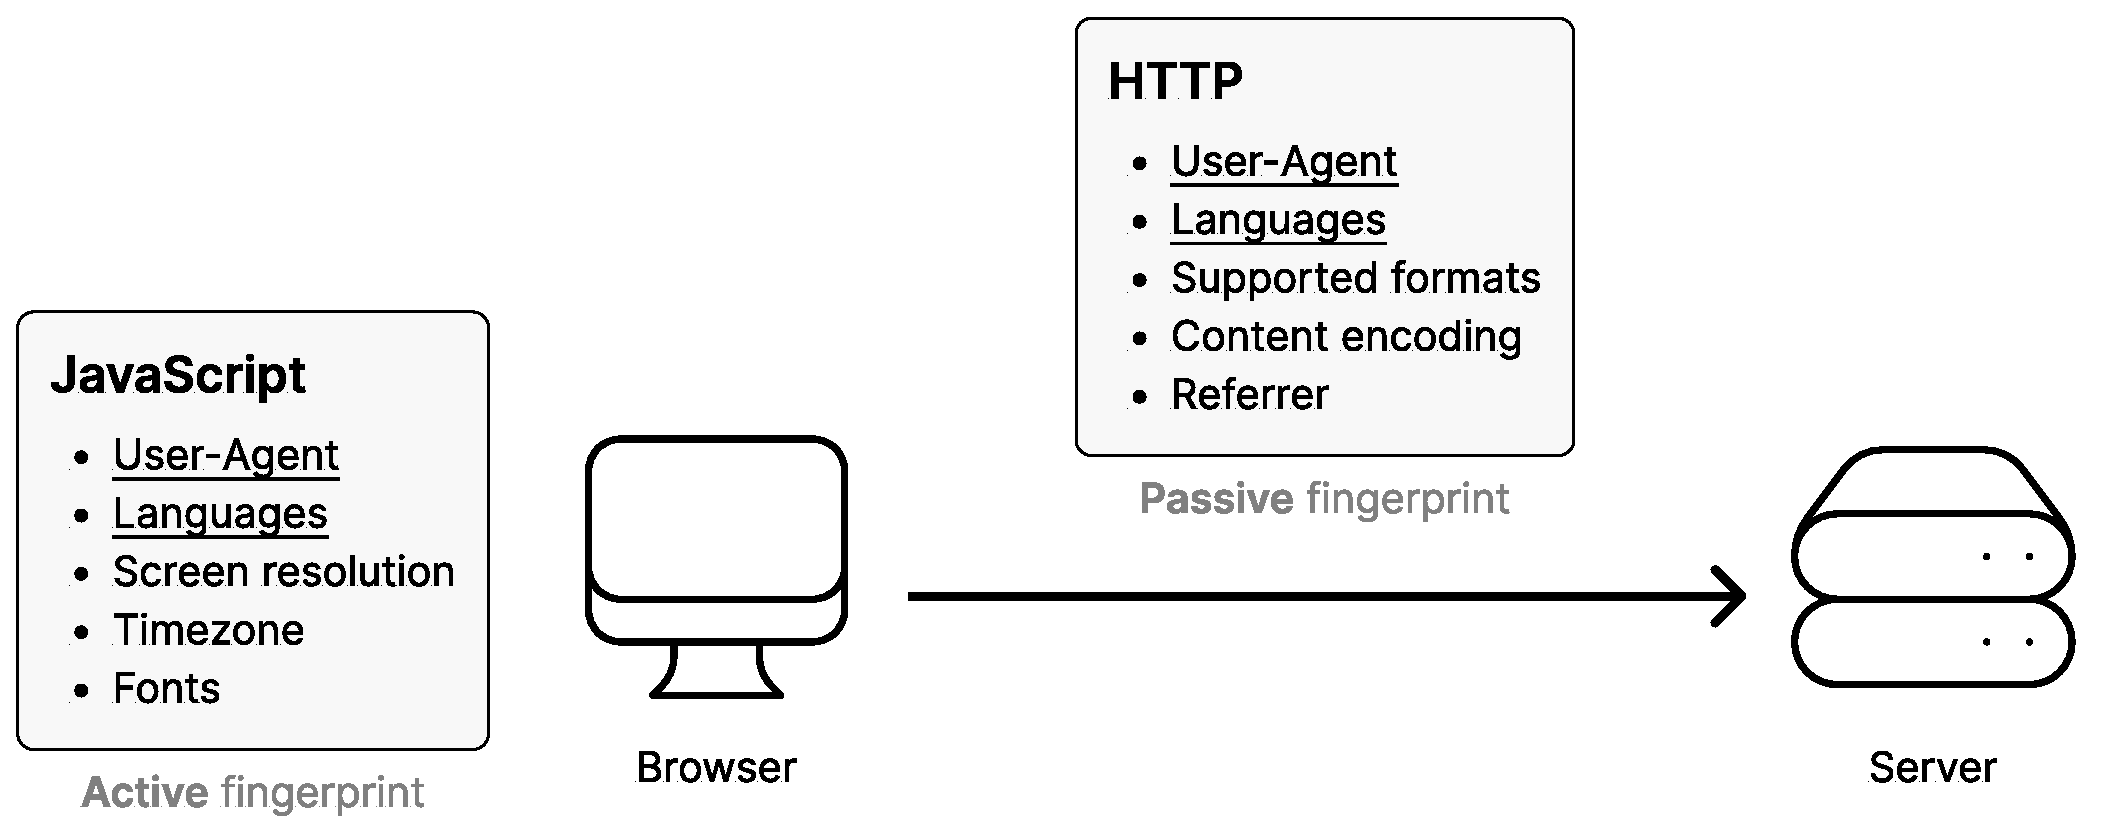
\includegraphics[width=\textwidth]{obrazky-figures/inconsistencies_schema}
    \caption{A scheme highlighting common properties obtainable with active and passive fingerprinting.}
    \label{fig:mesh1}
\end{figure}

Among the examples shown in tables \ref{Table:ActiveDataExamples} and \ref{Table:PassiveDataExamples} are characteristics with multiple data sources, namely the available memory, preferred languages, and the User-Agent string. Values of specific characteristics, such as the available memory or the User-Agent string, are one-to-one copies meaning the countermeasure algorithm can apply the same transformation to all data sources. However, this is not the case for the values of preferred languages characteristic. Preferred languages transferred in HTTP headers include the quality factor\footnote{Quality weights or quality values are used in HTTP headers to specify the order of priority in a comma-separated list (\url{https://developer.mozilla.org/en-US/docs/Glossary/Quality_values}).} for each language tag, but this value is absent in the version obtainable from the browser Web API. Tables Tables \ref{Table:ActiveDataExamples} and \ref{Table:PassiveDataExamples} illustrate this difference. An algorithm cannot apply the same transformation for all data sources as it has to be aware of these differences in representation.

Suppose a countermeasure algorithm misapplies the transformation to a data source, or the data source is left unchanged entirely. In that case, the fingerprinting application can detect and act on this attempt at fingerprint manipulation.

\section{Threats and opportunities of fingerprinting}
\label{FingerprintingThreatsOpportunities}

Fingerprinting is predominantly known for its often privacy-invading practices, but as with most things in our world, nothing is purely black and white. Fingerprinting brings good things (opportunities) and bad things (threats) to the table. This section discusses both, including example use cases.

\subsection{Threats}

Although fingerprinting is also used for good, it became popular mainly for reasons which could be considered a violation of privacy \cite{WP224Fingerprinting}. A person could be tracked for a long time until the device's characteristics change enough to affect the fingerprint. During this period, applications can show ads or products personalized to users based on browsing history and activity to boost their sales.

\subsection{Opportunities}

The ability to uniquely identify a device and transitively the user of the device allows third parties to change the behavior of their services and applications. Applications can use fingerprinting for payment fraud prevention and detection \cite{FingerprintJSUseCases} to prevent fraudsters from using stolen credit, debit, or checking data.

% -------------------------------------------------------------------- %

\chapter{JShelter}
\label{Section:JShelter}

In 2019, Martin Timko designed and implemented a proof of concept browser extension called \uv{Javascript Restricter} as a part of his master's thesis \cite{MatejTimkoDP}. Inspired by his work, Libor Polčák et al. \cite{JShelterPaper} created JShelter, a browser extension focused on fingerprinting prevention, limitations of rich web APIs, prevention of attacks connected to timing, and learning information about the device, the browser, the user, and surrounding physical environment and location. JShelter offers versions for three major browsers - Firefox, Chrome, and Opera.

\subsection{JavaScript Shield}

The pivotal protection feature of JShelter is the JavaScript Shield \cite{JShelterJavaScriptShield}, which modifies the behavior of the JavaScript environment of the browser. JShelter provides fake information to confuse fingerprinters and make webpage-triggered attacks harder or impossible.

The JavaScript Shield internally consists of small independent pieces of code called wrappers, which modify the original behavior of JavaScript APIs available in the browser. The behavior of wrappers can be categorized followingly \cite{JShelterJavaScriptShield}:

\begin{itemize}
	\item \textbf{Precision reduction}: The original value is unnecessarily precise for most use cases. JavaScript Shield modifies the values so that typical and essential use cases are unaffected.
	\item \textbf{Providing fake information}: Some wrappers provide fake information mostly to confuse fingerprinters. For example, canvas wrappers modify the image so that the exact instructions produce a different result in each session and for each domain.
	\item \textbf{Hiding information}: JavaScript Shield hides information from selected browser APIs that are generally unnecessary or have little use. Depending on the API, it might return an error, an empty value, or block the API completely.
\end{itemize}

To modify the values of the browser characteristics, the JavaScript Shield uses a technique called \emph{farbling} \cite{JShelterPaper}. This technique is based on the implementation of farbling in Brave \cite{BraveFingerprintingDefences2}, which has its roots in previous privacy research, including the PriVaricator \cite{PriVaricator} and FPRandom \cite{FPRandom}.

Farbling first deterministically generates a per-session, per-eTLD+1\footnote{eTLD+1 is a part of a domain name, including TLD, eTLD and one more domain part (More on \url{https://jfhr.me/what-is-an-etld-+-1/}).} seed. This seed is later used to slightly randomize the output of web APIs typically used for fingerprinting. The way a seed is generated makes cross-site and cross-session tracking difficult for fingerprinting applications.

% -------------------------------------------------------------------- %

\chapter{Design proposal}
\label{Chapter:Design}

This work aims to design and implement a new protective shield for the JShelter extension that can misrepresent information commonly used for passive fingerprinting. The first section of this chapter emphasizes the importance of avoiding alterations that could disrupt the user experience. Each of the following sections describes a selected HTTP header, proposes a modification to its value, the advantages and disadvantages of this modification, and necessary changes to the browser APIs to maintain consistency.

\section{Minimizing the impact on users}

It is crucial to remember that every modification the new protective shield will make to the outgoing requests can impact the response received from the server. For example, changing the preferred language reported by the browser to English would help make the fingerprint look more homogenous, as English is the prevalent language on the Internet. However, if the server reacts and returns a website in English, the user may need help understanding its content.

\section{HTTP header: User-Agent}
\label{SectionHTTPHeaderUserAgent}

The User-Agent request header is a characteristic string that lets servers and network peers identify the application, operating system, vendor, and/or version of the requesting user agent \cite{MDNHeaderUserAgent}. The value of this header varies depending on the operating system and browser type and version, making it an invaluable component of a fingerprint.

\bigbreak

\begin{lstlisting}[caption={An example of Chrome User-Agent string \cite{MDNHeaderUserAgent}.}, label={Listing:UserAgentChrome}]
Mozilla/5.0 (X11; Linux x86_64) AppleWebKit/537.36 (KHTML, like Gecko) Chrome/51.0.2704.103 Safari/537.36
\end{lstlisting}

\begin{lstlisting}[caption={An example of Safari User-Agent string (mobile version) \cite{MDNHeaderUserAgent}.}, label={Listing:UserAgentSafari}]
Mozilla/5.0 (iPhone; CPU iPhone OS 13_5_1 like Mac OS X) AppleWebKit/605.1.15 (KHTML, like Gecko) Version/13.1.1 Mobile/15E148 Safari/604.1
\end{lstlisting}

\medbreak

Figures \ref{Listing:UserAgentChrome} and \ref{Listing:UserAgentSafari} show examples of User-Agent strings of Chrome and Safari, which according to Statcounter GlobalStats \cite{StatcounterGlobalStats}, are the top two browsers with the highest market share of 64.62\% and 18.29\%, respectively. Statcounter GlobalStats is collecting statistics from more than 1.5 million sites with yearly views ranging from 5 to 6 billion. The examples above show that some browsers and operating systems have version numbers following the semantic versioning specification \cite{SemVerWebsite} or its variation. Semantic versioning in the most recent version 2 is composed of three segments separated by a dot (\uv{.}), where:

\begin{itemize}
	\item The first segment (\textbf{MAJOR}) is incremented when an incompatibility, such as a breaking API change, is introduced.
	\item The second segment (\textbf{MINOR}) is incremented when new functionality is added while still maintaining backward compatibility.
	\item The last segment (\textbf{PATCH}) is incremented for all other changes, for example, a bug fix or code refactoring.
\end{itemize}

From this, it is possible to make an observation. Given two version numbers that differ only in the last segment (\textbf{PATCH}), we know these software builds should have the same functionalities, meaning they should be indistinguishable for the user.

With this hypothesis, a change (either incrementing or decrementing) of the \textbf{PATCH} segment value would likely affect the fingerprint. However, at the same time, it is unlikely that the user would notice any difference.

The algorithm cannot change version numbers randomly, as this could create versions that were or never would be released. Instead, it would keep a list of previously released versions gathered from the changelog\footnote{Software products typically maintain a list of published versions. For example, the changelog of Chrome is available at \url{https://chromereleases.googleblog.com/search/label/Stable\%20updates}.} of the specific software product. The algorithm would then randomly select a suitable version from the list according to the requirements described above.

\subsection{Consistency}

The User-Agent string is also available through the \texttt{Navigator} interface, with the value being identical to the value transferred in the \texttt{User-Agent} HTTP header. It is necessary to apply the same transformation to the \texttt{Navigator.userAgent} to avoid inconsistencies.

\section{HTTP header: Accept}
\label{SectionHTTPHeaderAccept}

The Accept request HTTP header indicates which content types the client can understand, expressed as MIME types \cite{MDNHeaderAccept}. It is possible to add or remove MIME types to affect the fingerprint. However, the server may react to this modification and respond with an unexpected and incompatible response body.

\bigbreak

\begin{lstlisting}[caption={An example of Accept header contents \cite{MDNHeaderAccept}.}]
Accept: text/html, application/xhtml+xml, application/xml;q=0.9, image/webp, */*;q=0.8
\end{lstlisting}

\medbreak

A viable solution is to remove certain MIME types, which would not result in incompatibility, but only a slight performance hit. For example, it is possible to remove modern image formats such as \texttt{image/webp} and force the browser to use older image formats. This modification would affect the header value (and, transitively, the fingerprint value) without potentially breaking the website.

\subsection{Consistency}

Browsers no longer offer a standard API for quickly checking supported MIME types. The \texttt{Navigator.mimeTypes} API that partially allows this check has been deprecated and removed from the relevant web standards \cite{MDNNavigatorInterface}. A fingerprinting application could maintain a list of browser versions and supported MIME types which it would use to compare with the MIME types in the \texttt{Accept} HTTP 

Maintaining consistency but also checking the consistency is not trivial when it comes to the supported MIME types. Therefore, no browser API modifications are necessary.

\section{HTTP header: Accept-Language}
\label{SectionHTTPHeaderAcceptLanguage}

The Accept-Language request HTTP header \cite{MDNHeaderAcceptLanguage} indicates the natural language and locale that the client prefers. It is a list of preferred language tags separated by commas (\uv{,}). A language tag consists of a 2-3 letter base language tag that indicates a language, optionally followed by additional subtags separated by a dash (\uv{-}). The country or region variant (\texttt{en-US} or \texttt{fr-CA}) is the most common extra information stored in subtags. Language tags can optionally have a quality value (weight) represented by a decimal number separated from the tag by a semicolon (\uv{;}).

\bigbreak

\begin{lstlisting}[caption={An example of Accept-Language header contents \cite{MDNHeaderAcceptLanguage}.}]
Accept-Language: fr-CH, fr;q=0.9, en;q=0.8, de;q=0.7, *;q=0.5
\end{lstlisting}

\medbreak

Modifying this header is not straightforward because the server might respond with content in a different language if done wrong. One option is to change or remove language regions, as this information is often not crucial as the difference between language forms is usually manageable. For example, changing \texttt{en-US} (United States English) to \texttt{en-GB} (Great Britain English) might get noticed by users, but presumably, they would still understand the content.

\subsection{Consistency}

The client-preferred languages are also available through the \texttt{Navigator} interface under the \texttt{Navigator.languages} property. The languages are ordered the same way as in the \texttt{Accept-Language} header but without the quality value (weight). The first language is also extracted to the \texttt{Navigator.language}. Any change made to the \texttt{Accept-Language} HTTP header has to be reflected in these two properties of the \texttt{Navigator} interface.

\section{List of HTTP headers}

Another valuable characteristic used to create a fingerprint is a list of all headers present in a request. Most requests share standard headers such as those mentioned in previous sections \ref{SectionHTTPHeaderUserAgent}, \ref{SectionHTTPHeaderAccept}, and \ref{SectionHTTPHeaderAcceptLanguage}. However, it is common for requests to include less standard, even custom\footnote{Until 2012, developers tended to prefix custom headers with \uv{X-} to differentiate them from standardized headers, but this naming convention has been officially discouraged in RFC6648 \cite{RFC6648}.} headers.

\bigbreak

\begin{lstlisting}[caption={An example of a list of headers present in an HTTP request.}]
Accept, Accept-Encoding, Accept-Language, Connection, Cookie, Host, User-Agent
\end{lstlisting}

\medbreak

It is possible to add new headers to the HTTP request to alter the resulting fingerprint. If the newly added headers are custom, this change would likely not affect the response.

% For compilation piecewise (see projekt.tex), it is necessary to uncomment it
% \end{document}